%%% LyX 2.0.5.1 created this file.  For more info, see http://www.lyx.org/.
%%% Do not edit unless you really know what you are doing.
%\documentclass[12pt,english]{report}
%\usepackage{mathptmx}
%\renewcommand{\familydefault}{\rmdefault}
%\usepackage[T1]{fontenc}
%\usepackage[latin9]{inputenc}
%\usepackage[a4paper]{geometry}
%\setcounter{secnumdepth}{2} % Changed from 3 to 2. 0-chapter 1-section 2-subsection 
%\setcounter{tocdepth}{2} % Changed from 3 to 2. 0-chapter 1-section 2-subsection 
%\setlength{\parskip}{\medskipamount}
%\setlength{\parindent}{0pt}
%\usepackage{verbatim}
%\usepackage{pdfpages}
%\usepackage{graphicx}
%\usepackage{subfig} %% This package has to be here
%\usepackage{setspace}
%\usepackage{arabtex}
%\usepackage[numbers]{natbib}
%\usepackage{nomencl}
%\usepackage{paralist}
%\usepackage{amsthm}
%\usepackage{amsmath}
%\usepackage{amsfonts}
%\usepackage{etoolbox}
%\newtoggle{edit-mode}
%\togglefalse{edit-mode}  
%%\toggletrue{edit-mode}
%\iftoggle{edit-mode}{
%\geometry{verbose,tmargin=2cm,bmargin=2cm,lmargin=2cm,rmargin=6cm,headheight=1cm,headsep=1cm,footskip=1cm, marginparwidth=5cm}
%}{
%\geometry{verbose,tmargin=2cm,bmargin=2cm,lmargin=2cm,rmargin=2cm,headheight=1cm,headsep=1cm,footskip=1cm}
%}
%
%
%% Theorem Styles
%\newtheorem{theorem}{Theorem}[section]
%% Definition Styles
%%\theoremstyle{definition}
%\newtheorem{definition}{Definition}[section]
%\newtheorem{example}{Example}[section]
%\theoremstyle{remark}
%\newtheorem{remark}{Remark}
%
%\usepackage[linesnumbered]{algorithm2e}
%
%\begin{document}

%%%%%%%%%%% nomenclature %%%%%%%%%%
\nomenclature{KP}{Key Point}
\nomenclature{POI}{Point of Interest}
\nomenclature{HF}{Horizontal Fragment}
\nomenclature{FSP}{Final Segmentation Points}
\nomenclature{SSA}{Segmentation Selection Algorithm}
\nomenclature{FSS}{Forwards Segmentation Selection}
\nomenclature{BSS}{Backwards Segmentation Selection}
\nomenclature{BFSS}{Backwards-Forwards Segmentation Selection}
\nomenclature{GSS}{Greedy Segmentation Selection}
%%%%%%%%%%%%%%%%%%%%%%%%%%%%%%%%%%%

\chapter{Real-time Segmentation of On-line Handwritten Script}
\label{chap:strokes_segmentation}

In this chapter we describe a recognition-based segmentation approach for on-line Arabic script.
The segmentation is done in the stroke level while the stroke is being written, using the fast Arabic characters classification technique, described in Chapter \ref{chap:characters_classification}.

The proposed approach goes through three main stages.
The first stage is composed of two steps which are performed while the stroke is being scribed.
In the first step \emph{points of interest} (POIs) are nominated based on the morphological features of the stroke.
These POIs are the middle of the \emph{horizontal fragments} (HFs) and induce over segmentation of the stroke.
In the second step, once a POI is found, the classification information of sub-strokes which end with this POI is saved in a scoring matrix.
In the second stage, once the entire stroke is available, a rules-based process is used to refine the set of POIs and re-score the sub-strokes. 
Eventually, the system heuristically determines the final set of \emph{segmentation points} (SPs) based on the sub-strokes scoring. 

\begin{figure}
\centering
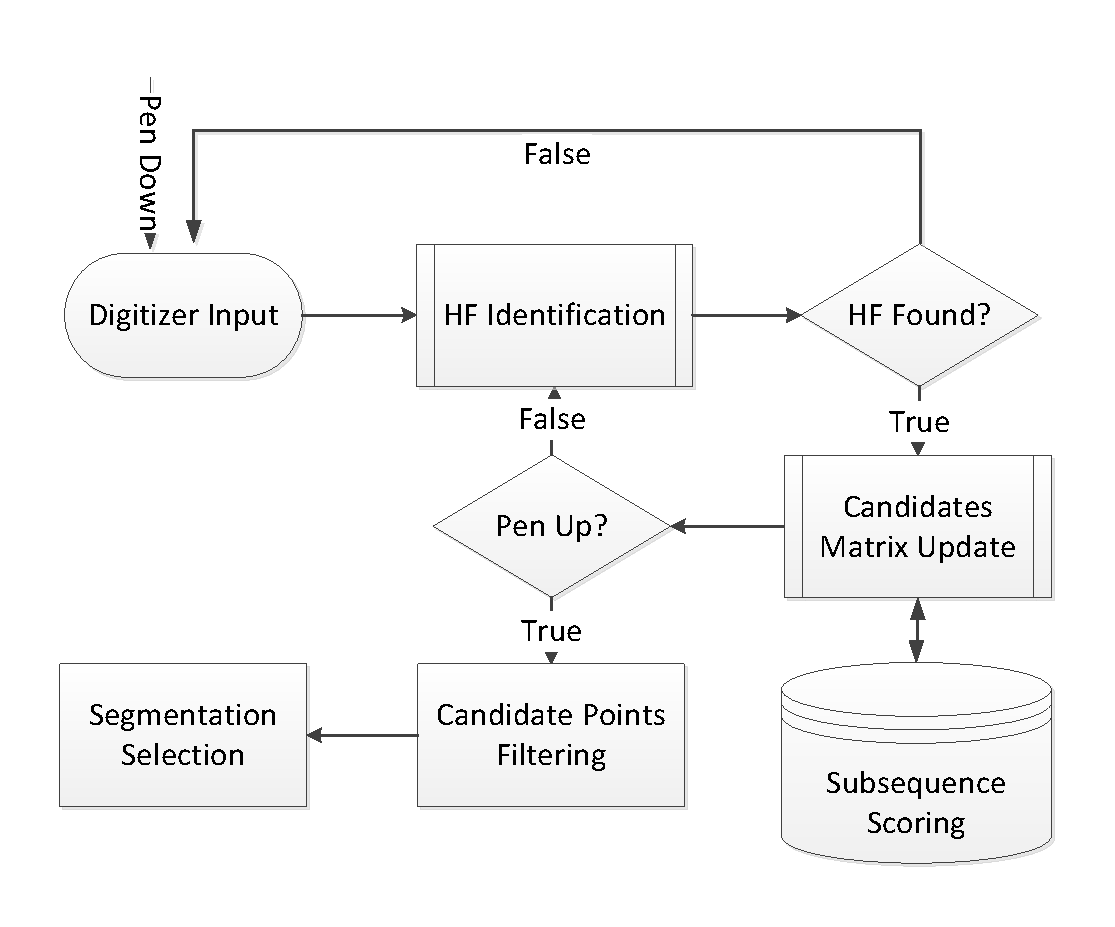
\includegraphics[width=0.8\textwidth]{./figures/system_flow}
\caption{High level visualization of segmentation flow.}
\label{fig:system_flow}
\end{figure}

%%%%%%%%%%%%%%%%%%%%%%%%%%%%%%%%%%%%%%%%%%%%%%%%%%%%%%%
\newpage{}
%%%%%%%%%%%%%%%%%%%%%%%%%%%%%%%%%%%%%%%%%%%%%%%%%%%%%%%

\section{First Stage: POIs Nomination and Sub-strokes Scoring}

\subsection{Horizontal Fragments Identification} 
In this stage, the system attempts to identify HFs that join pairs of connected letters. 
These handlers are horizontal, directed right to left and located near the baseline (see Figure  \ref{fig:horizontal_fragments}). 
Using a smoothed version of the trajectory helps the process to ignore undesired small horizontal regions that are frequently caused by the digitizer's imperfection.  
A point $p_{i}$ is defined as a "horizontal point" if the slope of the line $\overline{p_{i-1}p_{i}}$ is less than a pre-set value $\delta$, which was empirically tuned to $0.6$. 
The same exact value for this parameter was found independently in \cite{daifallah2009recognition}.

\begin{figure}
\centering
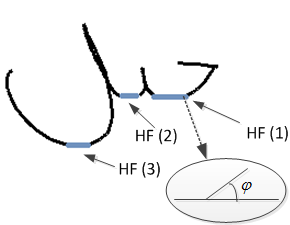
\includegraphics[width=0.3\columnwidth]{./figures/horizontal_fragments}
\caption{Horizontal fragments of the word \RL{jbl}.}
\label{fig:horizontal_fragments}
\end{figure}

HFs are continuously identified using the following process.
The first detected horizontal point is set as an "HF starting point". 
All the subsequent horizontal points are ignored until a non-horizontal point is detected, indicating the end of an HF sequence. 
This point is identified as an "HF ending point" and the medial point of an HF is marked as POI. 
POIs are potential SPs, thus, this process yields an over-segmentation of the stroke. 
While false positive SPs can be easily removed in a latter stage, missed SPs cannot be easily recovered. 
Therefore, in order to minimize the miss-rate, this process is delicate and allows false HFs to be detected.

Once an HF is detected the sub-stroke that spans from the previous POI to the POI of the current HF is checked to make sure they do not reside on the same HF. 
In case they do, both HFs are rejoined to a single HF. 
This is done to avoid fractions of the same HF to identified as multiple HFs. 
The merging is done by evaluating the complexity measurement across the two consequent HFs, see Figure \ref{fig:candidate_in_no_horizontal}.

\begin{definition}
\textbf{Complexity measure} is a value that indicates the curvature degree of a given 2-D trajectory $T=\{p_i\}_{i=1}^{n}$. 
Preprocessing steps, which include simplification and re-sampling, are required to ensure invariance under scaling and data imperfections. 
The complexity measure is calculated by summing the parameters $\alpha_{k}$ computed for each inner point $p_k$ in $T$ for $2 \leq k \leq n-1$, i.e., 
\begin{equation}
CM(T)=\sum_{k=2}^{n-1}{\alpha_k}.
\end{equation}
where the parameter $\alpha_{k}$ is defined as $\alpha_{k}=\frac{\pi-\phi_{k}}{\frac{\pi}{6}}$ and $\phi_k=\angle(\overline{p_{k-1}p_{k}},\overline{p_{k}p_{k+1}})$. 

\end{definition}

\begin{figure}
\centering
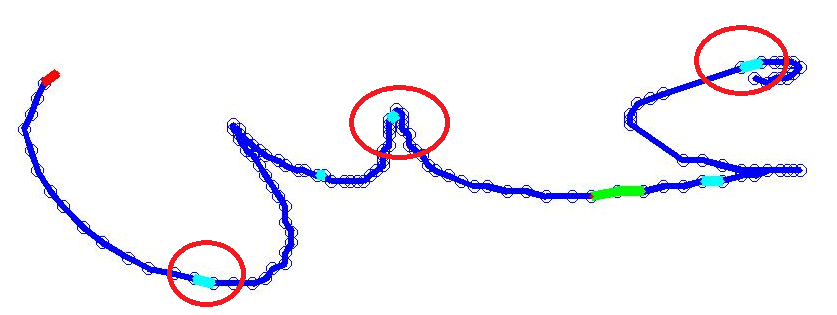
\includegraphics[width=0.3\textwidth]{./figures/candidate_in_no_horizontal}
\caption{The main body of the word \RL{`yn}. POIs are coloured in cyan. The green areas indicate merge between two subsequent HFs. 
Three types of false POIs can be seen: 1. A POI at the beginning of a stroke. 2. A POI that is caused by a bad HF. 3. A POI that resides in a letter's valley. }
\label{fig:candidate_in_no_horizontal}
\end{figure}

\subsection{Sub-strokes Scoring}
Let $S=\{p_{i}\}_{i=1}^{n}$ be a sequence representing a handwritten stroke in which $L$ POIs were detected. 
Let $KP=\{KP_{i}\}_{i=0}^{L+1}$ (Key points) be the ordered set of the POIs, in addition to the first and the last points of the stroke positioned as the first and the last items in the set.
Formally, we define: 
\begin{equation}
KP_{i} =\begin{cases}    1		, & \mbox{if } i=0 \\
					  POI_{i}	, & \mbox{if } 1\leq i \leq L \\
					       n    , & \mbox{if } i=L+1 
			\end{cases}				
\end{equation}
A sub-stroke $S_{i}^{j}$ is a sub-sequence of the stroke $S$ that starts at $KP_{i}$ and ends at $KP_{j}$, formally:
\begin{equation}
S_{i}^{j}=\{p_{k}\}_{k=KP_{i}}^{KP_{j}}; i<j
\end{equation}

We generate an upper triangular \emph{scoring matrix} $D\in\mathds{R}^{(L+1)\times (L+1)}$ where each cell $D_{i,j}$ represents the sub-stroke $S_i^j$. 
It contains the classification information and scoring, for the sub-strokes $S_i^j$, returned by the characters classification system described in Chapter \ref{chap:characters_classification}. 
The matrix $D$ is generated dynamically while the stroke is being written; adding a row and a column for each new detected POI. 
Imposing a locality constraint which narrows the band of the $D$ matrix above the main diagonal improved the efficiency of the process and the segmentation accuracy. 
Given a band width $B$ we fixed $D_{i,j}=\infty$ if  $j \leq i$ or $j-i>B$.
We argue that sub-strokes representing a letter will achieve, in most cases, better scoring, i.e., lower $D_{i,j}$ value than other sub-strokes.

\begin{figure}
\centering
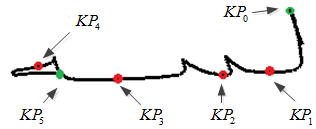
\includegraphics[width=0.4\textwidth]{./figures/candidate_points}
\caption{KPs of the word \RL{lbyh}. POIs are coloured in red. The first and last KPs are coloured in green. }
\label{fig:candidate_points}
\end{figure}

Using the relative location of the sub-stroke in the stroke, we restricted the classification process to search for similar samples feasible position databases.
As can be seen in Table \ref{table:subsequences_types}, we differentiate between four types of sub-sequences.
For each type, we indicate the set of databases that need to be examined, i.e., the possible letter positions the sub-stroke may represent. 
The relation between the cells in the matrix $D$ and the sub-stroke type is given in matrix $D_p$  (Equation \ref{eq:positions_matrix}). 
The type of the sub-stroke can be determined while the stroke is being scribed.
The last column and row are added on the "pen up" event.
\begin{table}
\centering
\renewcommand{\arraystretch}{1.3}
\caption{A mapping between the subsequence types and the possible letter positions. $S$ denotes a stroke containing $L$ POIs where $m>0$ and $k<L+1$.}
\begin{tabular}{c c c}
\toprule
  \textbf{Subsequence Symbol}     & \textbf{Subsequence Location}    & \textbf{Possible Letter Position}     \\
\midrule
  $\alpha$ & $S_0^{k}$      & $Ini$ or $Mid$      \\
  $\beta$  & $S_{m}^{k}$    & $Mid$               \\
  $\chi$   & $S_{m}^{L+1}$ & $Mid$ or $Fin$       \\
  $\delta$ & $S_0^{L+1}$    & All                 \\
\bottomrule
\end{tabular}
\label{table:subsequences_types}
\end{table}

\begin{equation}
D_{p}=
\left( 
\begin{array}{ccccccc}
\infty 	& \alpha & \alpha & \alpha  & \cdots & \alpha & \delta      \\
\infty  & \infty  & \beta   & \beta   & \cdots  & \beta  & \chi     \\
\infty  & \infty  & \infty   & \beta   & \cdots  & \beta  & \chi    \\
\vdots & \vdots & \vdots  & \vdots & \ddots  & \vdots & \vdots      \\
\infty  & \infty  & \infty   & \infty   & \cdots  & \beta  & \chi   \\
\infty  & \infty  & \infty   & \infty   & \cdots  & \infty  & \chi  \\
\infty  & \infty  & \infty   & \infty   & \cdots  & \infty  & \infty \end{array} \right)
\label{eq:positions_matrix}
\end{equation}\\

For a given input (sequence and position), the recognition system returns the $k$ nearest neighbours with different labelling, where the labelling is defined as the tuple (letter, position). In our implementation, we set $K=3$.

\begin{figure}
\centering
\renewcommand{\arraystretch}{1.1}
\begin{tabular}{ c | c  c  c  c  c }
\toprule
     & $1$ & $2$ & $3$ & $4$ & $5$ \\
\midrule
$0$
   & 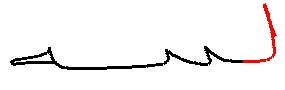
\includegraphics[width=0.16\linewidth]{./figures/substrokes/L}
   & 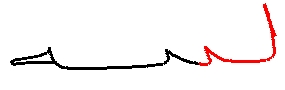
\includegraphics[width=0.16\linewidth]{./figures/substrokes/LB1}
   & 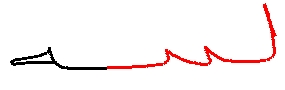
\includegraphics[width=0.16\linewidth]{./figures/substrokes/LB1B2}
   & $\varnothing$ & $\varnothing$ \\
$1$
   & $\varnothing$
   & 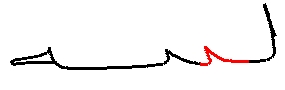
\includegraphics[width=0.16\linewidth]{./figures/substrokes/B1}
   & 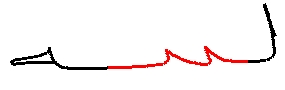
\includegraphics[width=0.16\linewidth]{./figures/substrokes/B1B2}
   & 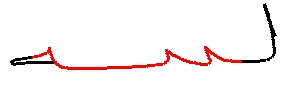
\includegraphics[width=0.16\linewidth]{./figures/substrokes/B1B2H1}
   & $\varnothing$ \\
$2$
   & $\varnothing$  & $\varnothing$
   & 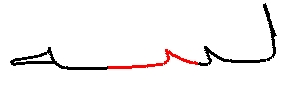
\includegraphics[width=0.16\linewidth]{./figures/substrokes/B2}
   & 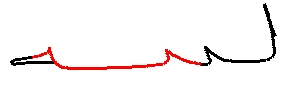
\includegraphics[width=0.16\linewidth]{./figures/substrokes/B2H1}
   & 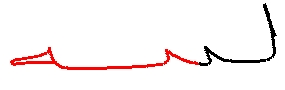
\includegraphics[width=0.16\linewidth]{./figures/substrokes/B2H} \\
$3$
   & $\varnothing$ & $\varnothing$ & $\varnothing$ 
   & 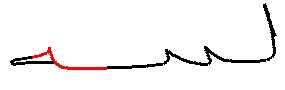
\includegraphics[width=0.16\linewidth]{./figures/substrokes/H1}
   & 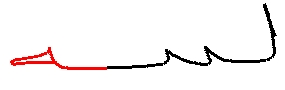
\includegraphics[width=0.16\linewidth]{./figures/substrokes/H} \\
$4$
   & $\varnothing$ & $\varnothing$ & $\varnothing$ & $\varnothing$ 
   & 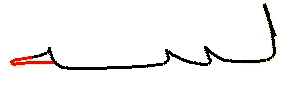
\includegraphics[width=0.16\linewidth]{./figures/substrokes/H2}\\
\bottomrule
\end{tabular}
\caption{
A tabular representation of the $D$ matrix that corresponds the KPs showed in Figure \ref{fig:candidate_points}. 
Each cell visually demonstrates the matching sub-stroke coloured in red.}
\label{table:substrokes_demo} 
\end{figure}



%%%%%%%%%%%%%%%%%%%%%%%%%%%%%%%%%%%%%%%%%%%%%%%%%%%%%%%
\newpage{}
%%%%%%%%%%%%%%%%%%%%%%%%%%%%%%%%%%%%%%%%%%%%%%%%%%%%%%%

\section{Second Stage: POI Filtering and Scoring Correction}
In this stage we re-score sub-sequences and eliminate redundant POIs based on the following rules:

\begin{compactitem}
	\item SPs should lie close to the baseline. 
	\item SPs do not reside in loops.
	\item The sub-stroke length should be proportional to the length of the containing stroke.
\end{compactitem}

Arabic text is written along an imaginary line called \emph{baseline}, with the majority of foreground pixels in this area.
It corresponds to the line upon which one would write on ruled paper. 
Many script recognition techniques use the baseline of the word in part of the recognition
process, for Arabic as well as for other languages.

Determining the baseline using the vertical projection histogram is a commonly used technique \cite{burrow2004arabic, bagdanov1997projection}.
Similarly, in this work, the system determines the baseline by calculating the vertical projection histogram of the re-sampled and normalized version of the stroke. 
The height of the stroke (y-axis) is partitioned into ten equi-length intervals. 
A POI is filtered out if it does not satisfy the following condition:
\begin{equation}
|POI_y-I_{max}| \leq 2 \cdot max{({|I|},0.15)} 
\end{equation}
where $POI_y$ represents the $y$-coordinate of the POI; $|I|$ is the length of an interval; and $I_{max}$ denotes the center of the most inhabited interval. 
In order to reliably determine the baseline, the detection algorithm is activated only after the fourth POI is found.
This process has proven to be very effective in eliminating challenging false POIs that reside in valleys of frequently used final Arabic letters, such as \RL{-q}, \RL{-s} and \RL{-n}. 
An example of such a POI can be seen in the letter \RL{-n} in Figure \ref{fig:candidate_in_no_horizontal}. 


The baseline is needed only to verify that the POIs are in a reasonable distance from it, therefore, imprecise valuation of the position or the direction of the baseline is tolerable.

\begin{figure}[b]
\centering

\includegraphics[width=0.8\textwidth]{./figures/baseline}
\caption{The position of the baseline corresponds to the largest peak of the vertical projection histogram \cite{burrow2004arabic}.}
\label{fig:candidate_in_no_horizontal}
\end{figure}

In order to identify SPs that resides inside a loop we have employed a Matlab package that includes an implementation for poly-line intersection algorithm \cite{legland2014geom2d}.

The third rule is used to penalize unreasonably low scoring given to small sub-strokes, which are unlikely to represent a letter. 
This is done by calculating the ratio of the sub-stroke length proportional to the entire stroke length.
For instance, it is common to add a small, hook-like, extension to the suffix of the letter \RL{d}. 
This extension may look very similar to the letter \RL{-a} during the stroke scribing; and thus under-scored, i.e., achieves a very good similarity measure by the recognition system, and eventually result in over-segmenting the letter \RL{d}. 

In some cases, POIs are incorrectly nominated on non-horizontal areas. 
This is caused due to noises in the data and the fact that the nomination is done while the word is being scribed. 
In a future work we will improve the filtering algorithm to handle such case.


%%%%%%%%%%%%%%%%%%%%%%%%%%%%%%%%%%%%%%%%%%%%%%%%%%%%%%%
\newpage{}
%%%%%%%%%%%%%%%%%%%%%%%%%%%%%%%%%%%%%%%%%%%%%%%%%%%%%%%

\section{Third Stage: Segmentation Selection}
The goal of this phase is to select the set of SPs among the POIs. 
This set will be referred to as the \emph{final segmentation points} (FSP). 
It is performed by finding the \emph{segmentation path} in $D$ with the best scoring possible. 
A segmentation path $\pi$ is an ordered subset of the KPs and must contain $KP_{0}$ and $KP_{L+1}$ as the first and the last points in the path.
$\Pi$ denotes the scoring of the segmentation path $\pi$. 
It is defined as the summation of the sub-sequences scoring in the segmentation path divided by the path length; this is done in order to prevent giving superiority to under-segmentations.

One can model the scoring matrix $D$ as a directed, edge-weighted graph $G=(V,E)$, for which a path from vertex $KP_0$ to vertex $KP_{L+1}$ defines a possible segmentation. 
It can be experimentally validated that finding the shortest path in $G$ (from $KP_0$ to $KP_{L+1}$) does not necessarily obtain the optimal segmentation, and in some cases, produces under-segmentation of the stroke. 
It is because the shortest path is a global property, which may prefer a highly weighted shortcut path over a path that consists of several low weighted fragments; in cases where the accumulative weight of the fragmented path is larger than the shortcut path.
However, greedily selecting the outgoing edge with the minimal weight will mostly return a better segmentation.

Several \emph{segmentation selection algorithms} (SSAs) for finding the best segmentation path are proposed in this work.
Here we describe two algorithms that were given the names \emph{Forwards Segmentation Selection} (FSS) and \emph{Backwards Segmentation Selection} (BSS) which operate quite similarly. 
A pseudo-code of FSS algorithm can be seen in Algorithm \ref{alg:fss}. 
FSS starts with the first point, $KP_0$, advancing toward the end of the stroke. 
In Each step, it tries to find the next best KP by selecting the adjacent subsequence $S_i^j$ with the best scoring (as can be seen in line 5). 
BSS operates similarly but starts from the last point and advances toward the beginning of the stroke. 
The main drawback of these two algorithms is that FSS tends to under-segment the suffix of the stroke and BSS tends to under-segment the stroke's prefix.

In an attempt to overcome the aforementioned drawbacks, a third SSA is proposed, and given the name \emph{Backwards-Forwards Segmentation Selection} (BFSS). 
As can be seen in Algorithm \ref{alg:bfss}, it combines both FSS and BSS. 
BFSS operates from the sides of the stroke toward the center. In every iteration, it selects two candidate points to include to the segmentation path.

\begin{algorithm}[h]
$\pi = \{0\} $\;
$i=0$\;
$sum=0$\;
\While{$i<L+1$}
{
	$j = \mathop {\arg \min }\limits_k \left( {D\left( {i,k} \right)} \right)$\;
	$\pi = \pi \cup \left\{ j \right\}$\;
	$sum = sum + D\left( {i,j} \right)$\;
	$i=j$\;
}
\caption{Forwards Segmentation Selection (FSS) algorithm.}
\label{alg:fss}
\end{algorithm}

\begin{algorithm}[h]
$\pi = \{0,L+1\}$\;
$kp_{a}=0$\;
$kp_{b}=L+1$\;
\While{$kp_{a}<kp_{b}$}
{
	$kp_{a,next} = \mathop {\arg \min}\limits_k (D(kp_a,k))$\;
	$\pi = \pi \cup \{kp_{a,next}\}$\;
	$kp_{a}=kp_{a,next}$\;
	
	$kp_{b,next} = \mathop {\arg \min}\limits_k (D(k,kp_{b,next}))$\;
	$\pi = \pi \cup \{kp_{b,next}\}$\;	
	$kp_{b}=kp_{b,next}$\;
}
\caption{Backwards-Forwards Segmentation Selection (BFSS) algorithm.}
\label{alg:bfss}
\end{algorithm}

\begin{algorithm}[h]
$\pi = \{0,L+1\}$\;
\While{$D \neq [\infty]^{(L+1)\times (L+1)}$}
{
	${s,e} = \mathop {\arg \min}(D)$\;
	$\pi = \pi \cup \{s,e\}$\;
	$sum = sum + D(s,e)$\;
	$UpdateMatrix(D,s,e)$\;
}

\caption{Greedy Segmentation Selection (GSS) algorithm.}
\label{alg:gss}
\end{algorithm}
  
The last algorithm was given the name \emph{Greedy Segmentation Selection} (GSS) and is described in Algorithm \ref{alg:gss}.
GSS operates differently. In every iteration, the cell with the lowest (best) scoring is selected. 
Once a cell $D_{i,j}$ is selected, since it represents the sub-stroke $S_{i}^{j}$, both $KP_{i}$ and $KP_{j}$ are added to the FSP, and every cell corresponding to a subpart of the sub-stroke $S_{i}^{j}$ is removed by setting its corresponding scoring value in the matrix $D$ to $\infty$; in order to avoid those sub-strokes to be selected in a later iteration. In Algorithm \ref{alg:gss}, the notation $[\infty]^{(L+1)\times (L+1)}$ indicates a matrix that all it's cells are set to $\infty$.
Performance evaluation of the mentioned SSA is provided in Section \ref{subsec:ssa_performance}.

%%%%%%%%%%%%%%%%%%%%%%%%%%%%%%%%%%%%%%%%%%%%%%%%%%%%%%%
\newpage{}
%%%%%%%%%%%%%%%%%%%%%%%%%%%%%%%%%%%%%%%%%%%%%%%%%%%%%%%

\section{Experimental Results}
\label{sec:segmentation_results}
Comparing the performance of the real-time segmentation approach described in this work to results obtained by related researches is difficult due to the different experimental settings, databases and methodology; not to mention the different measures used to present the results. 
The usage of the ADAB database, instead of a self-collected database, standardize and reinforces our results. 
In Table \ref{table:general_stats}, we provide basic statistics of our sample set. 
Table \ref{table:segmentation_results} summarizes the system's performance.

\begin{table}[b]
\renewcommand{\arraystretch}{1.2}
\centering
\caption{Segmentation system testing set.}
\begin{tabular}{ c c }
\toprule
  Number of test samples (city names) & 319 \\
  Number of WPs & 1148 \\
  Number of Strokes & 1237 \\
\bottomrule
\end{tabular}
\label{table:general_stats} 
\end{table}


\begin{table}[b]
\renewcommand{\arraystretch}{1.2}
\centering
\caption{Segmentation performance.}
\begin{tabular}{cc||cc}
\toprule
  Strokes SR &  83\% & Missing SPs  & 14.7\%\\
  Strokes RR &  78\% & Invalid SPs  & 11\%\\
  \# true SPs & 1081 & SPs precision & 88.6\%\\ 
  Valid SPs  & 85.3\% & SPs recall  &  85.3\%\\
  \bottomrule
\end{tabular}
\label{table:segmentation_results}
\end{table}


\subsection{Validation}
\label{subsec:validation}
Related researches usually use a human expert to validate the accuracy of the SPs. However, in this work, we applied an automatic validation process using the ground truth information provided by the database. We discriminate between three types of final SPs. A final SP is classified as true positive if the complexity measure between the identified point and a true SP is less than a pre-set threshold; otherwise, it is classified as false positive. A false negative (miss), is the case when the system failed to identify a true SP. The different types of SPs can be seen in Figure \ref{fig:sp_types}.
The validation process was tested on several sets and found to be highly reliable.

\begin{figure}
\centering
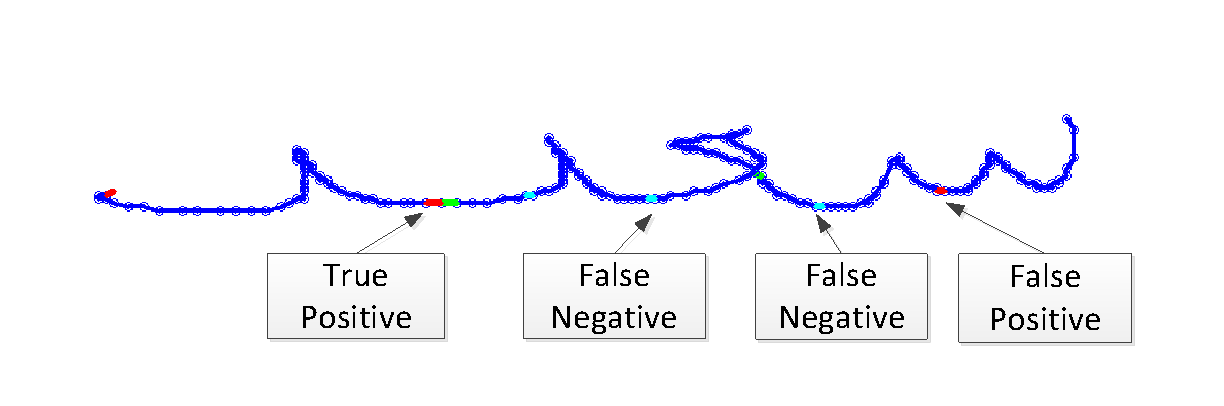
\includegraphics[width=0.6\textwidth]{./figures/sp_types}
\caption{POIs classification.}
\label{fig:sp_types}
\end{figure}

\subsection{Analysis}
In this section we discuss common cases of incorrect segmentation.\\
\subsubsection{Over-segmentation}
\begin{itemize}
\item Several Arabic letters contain a horizontal region in their initial form which does not accommodate a SP, see Figure \ref{fig:candidate_in_no_horizontal}. 
We overcame this problem by adding the following rule: a POI is nominated only if the sub-stroke that spans from the beginning of the stroke to the POI has a high complexity measure.
\item Over-segmentation can also be caused by typing a letter in unusual form where it is spanned over several strokes. 
It happens mostly in the letter \RL{-m-}, \RL{-m} and in rare cases in the letter \RL{-.h-}. This issue will be addressed in a future work.
\end{itemize}

\begin{figure}
\centering
        \subfloat[]{
            \label{fig:letters_same_body_1}
            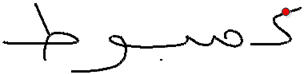
\includegraphics[width=0.3\textwidth]{./figures/oversegmentation_begin_1}
        }
        \subfloat[]{
           \label{fig:letters_same_body_2}
           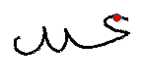
\includegraphics[width=0.15\textwidth]{./figures/oversegmentation_begin_2}
        }        
    \caption{Samples of false POI at the beginning of the stroke.}
   \label{fig:oversegmentation_begin}
\end{figure}


\begin{figure}
\centering
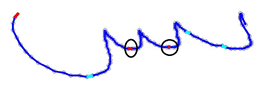
\includegraphics[width=5cm]{./figures/oversegmentation_s}
\caption{Over-segmentation in the letter \RL{-s-} .}
\label{fig:oversegmentation_s}
\end{figure}

\subsubsection{Under-segmentation}
\begin{itemize}
\item Letter pairs that are not separated by HFs cause the system to miss POIs. This was partially solved by extending the notion of a letter to include such pairs. For example the pair \RL{lm} and \RL{l.h}.
\item In some cases, HFs were identified correctly but the corresponding POI were not selected in the third stage. This may result from nomination of a candidate point on correct horizontal segment but in a late fraction of the segmentation fragment which result in a low scoring and thus not being selected by the SSA. This issue usually occurs in the letter \RL{w} in its final position, see Figure \ref{fig:undersegmentation_w}.
\end{itemize}

\begin{figure}
\centering
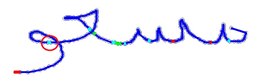
\includegraphics[width=5cm]{./figures/undersegmentation_w}
\caption{An example of a late POI in the letter \RL{w}.}
\label{fig:undersegmentation_w}
\end{figure}

We have noticed that the absolute majority of the false negative (missed) SPs were actually identified as POIs in the first stage, but were not selected by the SSA.
In addition, differentiating between the main body of the letter \RL{-s-} and the main body of two consecutive \RL{-b-} letters is possible only when considering the additional strokes, thus both cases were considered to be correct.

\subsection{Segmentation Selection Algorithms Performance}
\label{subsec:ssa_performance}
It is apparent from the data in Table \ref{table:ss_algorithms_results}, that the SSA has a crucial effect on the system's performance. 
We tested several combinations of two SSAs in which the FSP is found by executing both SSAs independently and selecting the segmentation path with the smallest scoring.

\begin{table}
\centering
\caption{Comparing the different SSAs performance. A combination of two algorithms is denoted by $\oplus$.}

\begin{tabular}{c c c c c}
\toprule
\textbf{SSA} & \textbf{WP segmentation} & \textbf{WP recognition} & \textbf{SP precision} & \textbf{SP recall}\\
             & \textbf{rate}            & \textbf{rate}           &                       &\\            
  \midrule
  FSS & 76\% & 70\% & 85\% & 78\% \\ 
  BSS & 79\% &  73\% & 84\%& 81\% \\
  BFSS & 78\% & 72\% & 84\% & 80\%\\ 
  GSS & 80\% & 74\% & 81\% & \bf{94}\% \\ 
  FSS$\oplus$BSS & \bf{82}\% & \bf{76}\% & \bf{89}\% & 82\%\\  
  GSS$\oplus$BFSS & 81\% & 75\% & 83\% & 90\% \\
  \bottomrule
\end{tabular}
\label{table:ss_algorithms_results} 
\end{table}

\subsection{Sample-set Size and Distribution}
The letters is our training set are extracted from a database with a limited words diversity, thus, the distribution of the samples between the different classes is imbalanced. 
On one hand, it can be regarded as an advantage; since, the training set distribution reflects the a-priory probability of a letter appearance in the test set. 
On the other hand, a highly imbalanced training set is known to negatively affect many classification algorithms.
In the following experiment, we measure the effect of a large and imbalanced training set on the WP segmentation and recognition rates. 
It is done by gradually increasing the maximal allowed number of samples per class (letter and position).
 
The graph in Figure \ref{fig:num_letter_impact} shows convergence of the system's performance when the maximal number of samples is larger than 200 per class. 
Nevertheless, a miniature degradation is apparent, which is caused, probably, due to the increasing imbalance in the distribution of the training set.
In addition, it is evident that the recognition rate is more sensitive to small training set than the segmentation rate.

\begin{figure}
\centering
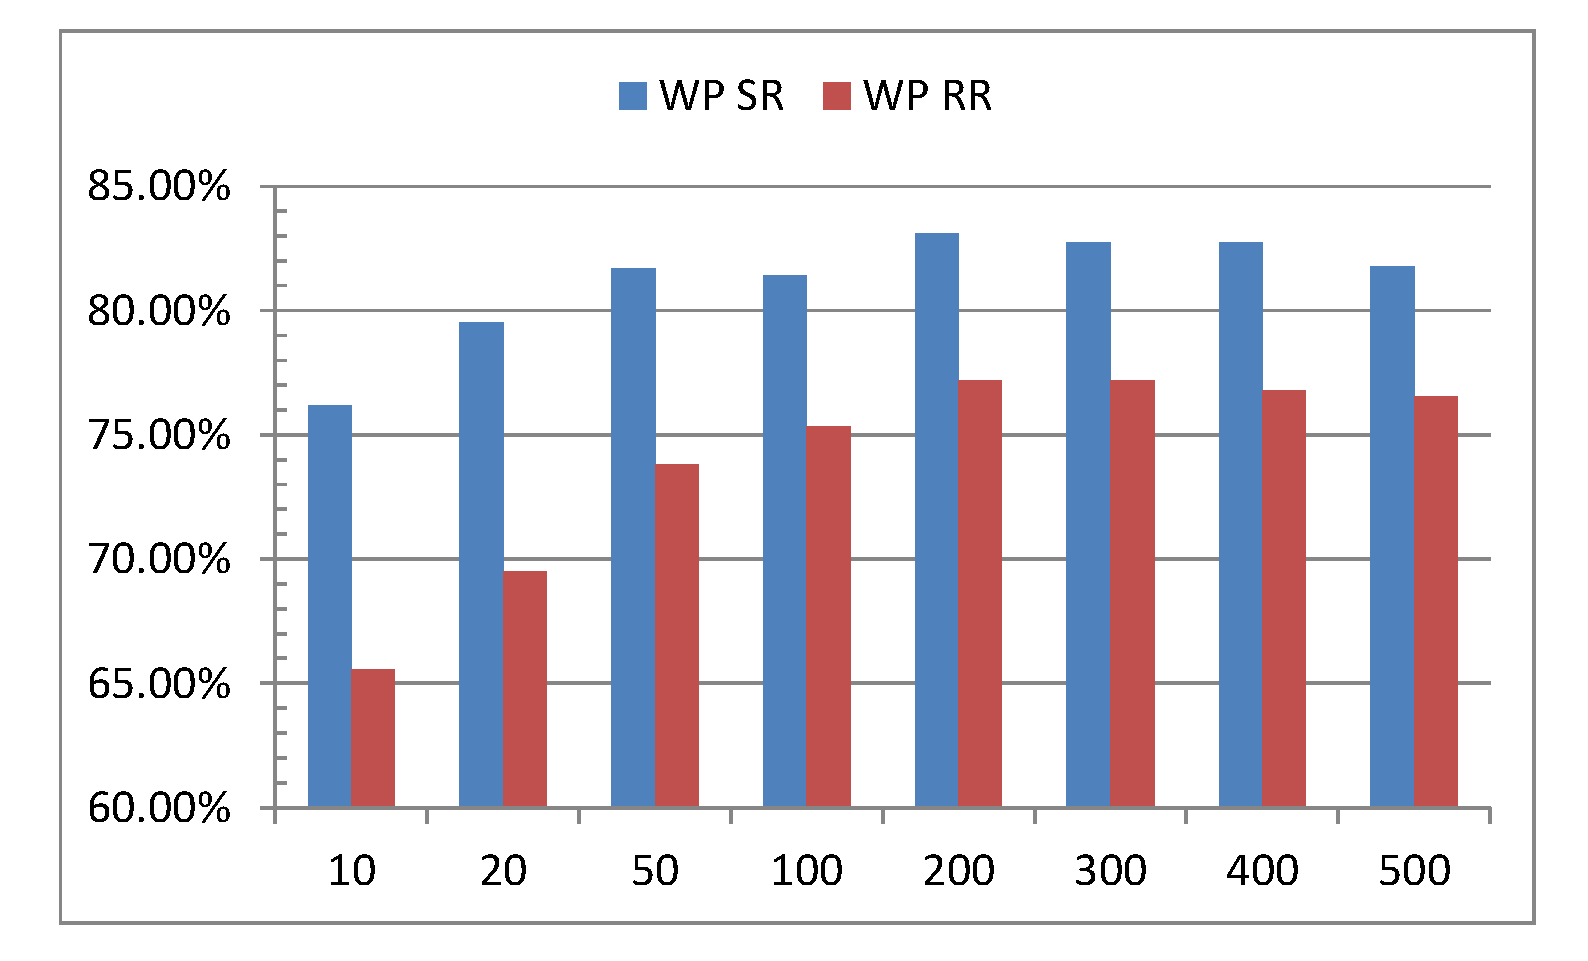
\includegraphics[width=0.7\textwidth]{./figures/num_letter_impact}
\caption{The impact of increasing the maximal number of samples per class on the segmentation and recognition rates.}
\label{fig:num_letter_impact}
\end{figure}

%%%%%%%%%%%%%%%%%%%%%%%%%%%%%%%%%%%%%%%%%%%%%%%%%%%%%%%
\newpage{}
%%%%%%%%%%%%%%%%%%%%%%%%%%%%%%%%%%%%%%%%%%%%%%%%%%%%%%%

\section{Holistic WPs Recognition using Characters Classification Information}
\label{sec:wps_recognition}
As mentioned earlier, the segmentation and classification information obtained by a real-time segmentation system, can be used to significantly reduce the potential dictionary size and accelerate a later holistic recognition process as follows:
\begin{compactitem}
\item In an open-vocabulary environment, the classification information can be employed to dynamically build a class of different shapes for all possible WPs.
\item In a closed-vocabulary environment, a holistic recognition approach can be limited to consider valid combination that appear in the vocabulary. 
\end{compactitem}

In this section we evaluate the recognition accuracy that can be obtained in the an open-vocabulary environment.
Following the real-time segmentation process, the $10$ top scored candidates of each character are recorded. 
These shapes are used to generate a complete list of all possible shape concatenation of the retrieved candidates. 
The obtained candidates represent different shapes of the same letter producing multiple shapes of the same WP. 
The cardinality of the generated list is $10^p$ where $p$ is the predicted number of characters in the WP using the segmentation process. 
The large size of the generated list, which may exceed $10,000$ shapes, requires a similar process of embedding and dimensionality reduction, as described above, to generate a short list of candidates. 
The short list of candidates in the next step is matched against the queried WP using the original expensive and more accurate matching process. 
Using the proposed approach, the $10$ top WPs results yield a $98.1\%$ recognition rate. 
The recognition rate of the first top candidate dropped down to $90.8\%$. 
Using a voting process within the top five results gave a $94.7\%$ recognition rate. 

Analysing the failures of the misclassified samples shows that most recognition errors occur as a result of misclassifying a single character. 
In most cases the misclassified character is confused with a character having a very similar shape, which can be corrected using information retrieved by the associated additional stroke, such as the case of the letter \RL{-l} and the letter \RL{-n} in their handwritten form.


%\bibliographystyle{plainnat}
%\bibliography{references}
%
%\end{document}